\documentclass[11pt,a4paper]{article}
\usepackage[margin=2.2cm]{geometry}
\usepackage{graphicx,booktabs,amsmath,xcolor,float}
\usepackage[hidelinks]{hyperref}
\usepackage[font=small,labelfont=bf]{caption}
\newcommand{\pc}{p_c}
\title{Without the cross-modal block: can the bias ($c$, $d$) be recovered,\\ and what the noise calibration really measures}
\author{av-dur v2 \quad 29 October 2026}
\date{}
\begin{document}
\maketitle
\vspace{-1.5em}

\section*{Summary}
\begin{enumerate}
\item \textbf{$c$ cannot be recovered from the main experiment.} This holds whatever is known about $\sigma_A$. Recovered and true values correlate at $r \le 0.38$ (often near 0). The error (RMSE 0.40--0.67) is three to four times the spread of the true values (SD 0.14), and 10--37\% of fits end at a bound. Under fusion, $c$ cancels exactly; under CI and switching it acts only through the perceived discrepancy. \emph{Fix $c = 0$ in the bimodal fits.}
\item \textbf{$d$ can be recovered only for fusion observers, and only when $\sigma_A$ and $\sigma_V$ are known very precisely.}
  \begin{itemize}
  \item With a log error of 0.05 on both: $r = 0.83$, RMSE 0.19 (true SD 0.27).
  \item With a log error of 0.15: $r = 0.65$, RMSE 0.35, so already worse than guessing the mean.
  \item For CI and switching observers, never ($r \le 0.43$, RMSE $\ge 0.44$): $d$ trades off against $\pc$ and $p_\text{switch}$.
  \end{itemize}
  A per-participant $d$ needs the cross-modal block.
\item \textbf{Free bias terms make model selection worse,} even though every simulated participant had a bias. With $\sigma_A$ known (log error 0.15), the right model is found for 92\% without bias terms, 86\% with $d$, and 80\% with $c$ and $d$ (fusion only 57\%). \emph{Compare models with the no-bias fits.}
\item \textbf{Ignoring $d$ costs little in $\pc$.} The $\pc$ error grows by about 0.2 per unit of $d$: participants with $d < 0$ get $\pc$ about 0.11 too low, and $d$ between 0 and 0.6 is nearly unbiased. The overall RMSE is the same with and without $d$ in the fit (0.155 vs 0.158).
\item \textbf{The big gain is elsewhere: tie $\sigma_A$ to the unimodal auditory block,} as your joint fit does. Model recovery rises from 83\% to 92\% (switching 77\%\,$\to$\,97\%, CI 88\%\,$\to$\,93\%, fusion 83\%\,$\to$\,86\%), and the $\pc$ RMSE falls from 0.167 to 0.155 (0.127 at log error 0.05).
\item \textbf{The catch: the unimodal block's $\sigma_A$ is a mixture of two orders} (Section~\ref{sec:order}). In loud noise most participants are near chance with the test first and sharp with it second. Noise barely changes discrimination with the test second (P105: $\sigma$ 0.12 at noise 0.5, 0.22 at 2.0). A single $\sigma_A$ per noise level averages two very different things, and the noise calibration overshot for P103 and P105 because of it. It is now capped at 1.2.
\end{enumerate}

\paragraph{Suggested analysis plan.}
\begin{itemize}
\item \textbf{Main fit:} the joint fit with $\sigma_A$ and $\sigma_V$ shared with the unimodal blocks, no bias terms, models compared by AIC.
\item \textbf{Sensitivity check:} refit with $d$ free, or fixed at a group value, and confirm that model choice and $\pc$ stay the same.
\item \textbf{If $c$ or $d$ per participant matter scientifically:} only the cross-modal block measures them. With 3 standards, $d$ is measured with an SE of 0.08--0.18 (28 Oct report). It is still in the launcher as an option. A group-level (hierarchical) $d$ would be the alternative.
\item \textbf{Before relying on shared $\sigma_A$:} decide how to handle presentation order (a $\sigma_A$ per order, or a model of the first interval), and check whether the bimodal data show the same order dependence.
\end{itemize}

\section{What was simulated}\label{sec:sim}
\texttt{bias\_recovery.py}; analysis and figures in \texttt{bias\_analyse.py}.
\begin{itemize}
\item \textbf{Participants.} 346 simulated participants: 116 causal inference (CI), 115 forced fusion, 115 switching. Model parameters are drawn as in the 28 Oct report: $\lambda \sim U(0.001, 0.1)$, $\sigma_{A,\text{low}} \sim U(0.12, 0.45)$, $\sigma_{A,\text{high}} \sim U(0.55, 1)$, $\sigma_V \sim U(0.3, 1)$, $\pc$ and $p_\text{switch} \sim U(0.1, 0.9)$.
\item \textbf{Bias, in both intervals:} $\ln \hat v = \ln v - c_\text{noise} - d \ln(v / 0.5)$, with $c_\text{low} \sim U(0, 0.5)$, $c_\text{high} \sim U(-0.1, 0.4)$ and $d \sim U(-0.3, 0.6)$. These ranges come from the cross-modal blocks of P101, P102 and P104: $c$ 0.06--0.50, $d$ $-0.23$ to 0.60.
\item \textbf{Main experiment as it now runs:} 9 conflicts ($\pm$450\,ms) $\times$ 2 noise levels, a 2D1U and a 1D2U staircase per condition, easy trials, whole frames at 120\,Hz. 70 trials per condition, 1260 in all. (106 trials per condition, run only with $\sigma_A$ free, gave the same results.)
\item \textbf{Fits:} each model fitted three ways by BADS: no bias; $d$ only; $c_\text{low}$, $c_\text{high}$ and $d$. The biased fits also start from the no-bias solution, so they never fit worse.
\item \textbf{What the unimodal blocks contribute} (the three scenarios):
  \begin{itemize}
  \item \emph{$\sigma_A$ free:} $\sigma_A$ is fitted from the bimodal data alone. $\sigma_V/(1-d)$, the visual $\sigma$ the unimodal block measures, is fixed at its true value $\times\, e^{N(0, 0.2)}$.
  \item \emph{$\sigma_A$ known, log error 0.15 or 0.05:} each $\sigma_A$ is estimated as the true value $\times\, e^{N(0, \text{err})}$ and added to the likelihood as a Gaussian penalty on $\ln\sigma_A$, which approximates the unimodal block's likelihood in a joint fit. $\sigma_V$ is fixed with the same log error.
  \end{itemize}
  All three scenarios use the same simulated data. For comparison, the QUEST+ simulations (\texttt{analysis/quest\_simulation\_results}) put the log error of a 100 + 20-trial block at about 0.23 and of the 150 + 20 used from 29 Oct at about 0.20, so 0.15 is optimistic (it would take about 300 trials per condition).
\end{itemize}

\section{Results}
\subsection{$c$ is not identified}
\begin{figure}[H]
\centering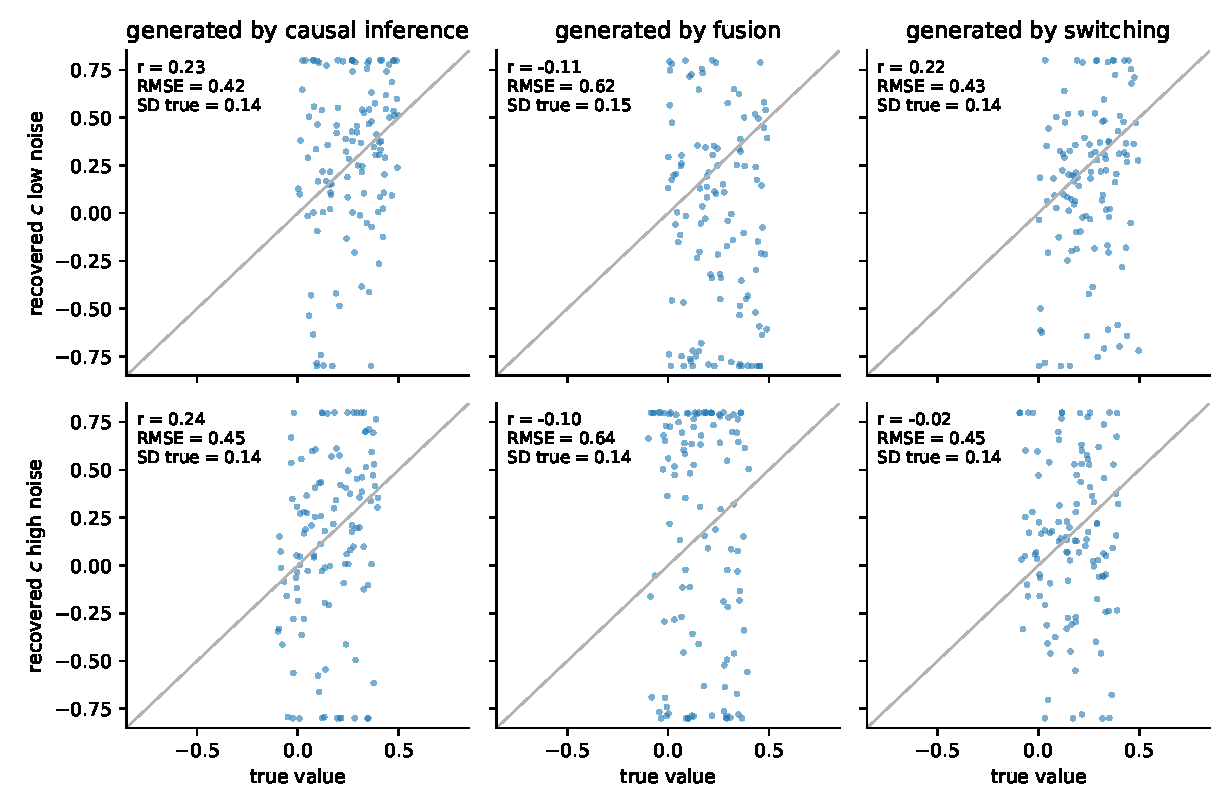
\includegraphics[width=0.6\linewidth]{fig_bias_c.pdf}
\caption{Recovered vs true $c$, from the fit with $c$ and $d$ free, by the generating model; $\sigma_A$ known (log error 0.15). The other scenarios look the same: $r$ between $-0.11$ and $0.38$, RMSE 0.40--0.67 against a true SD of 0.14. Values beyond $\pm$0.8 are at the bounds.}
\end{figure}

\subsection{$d$: fusion observers only, and only with precise $\sigma$s}
\begin{figure}[H]
\centering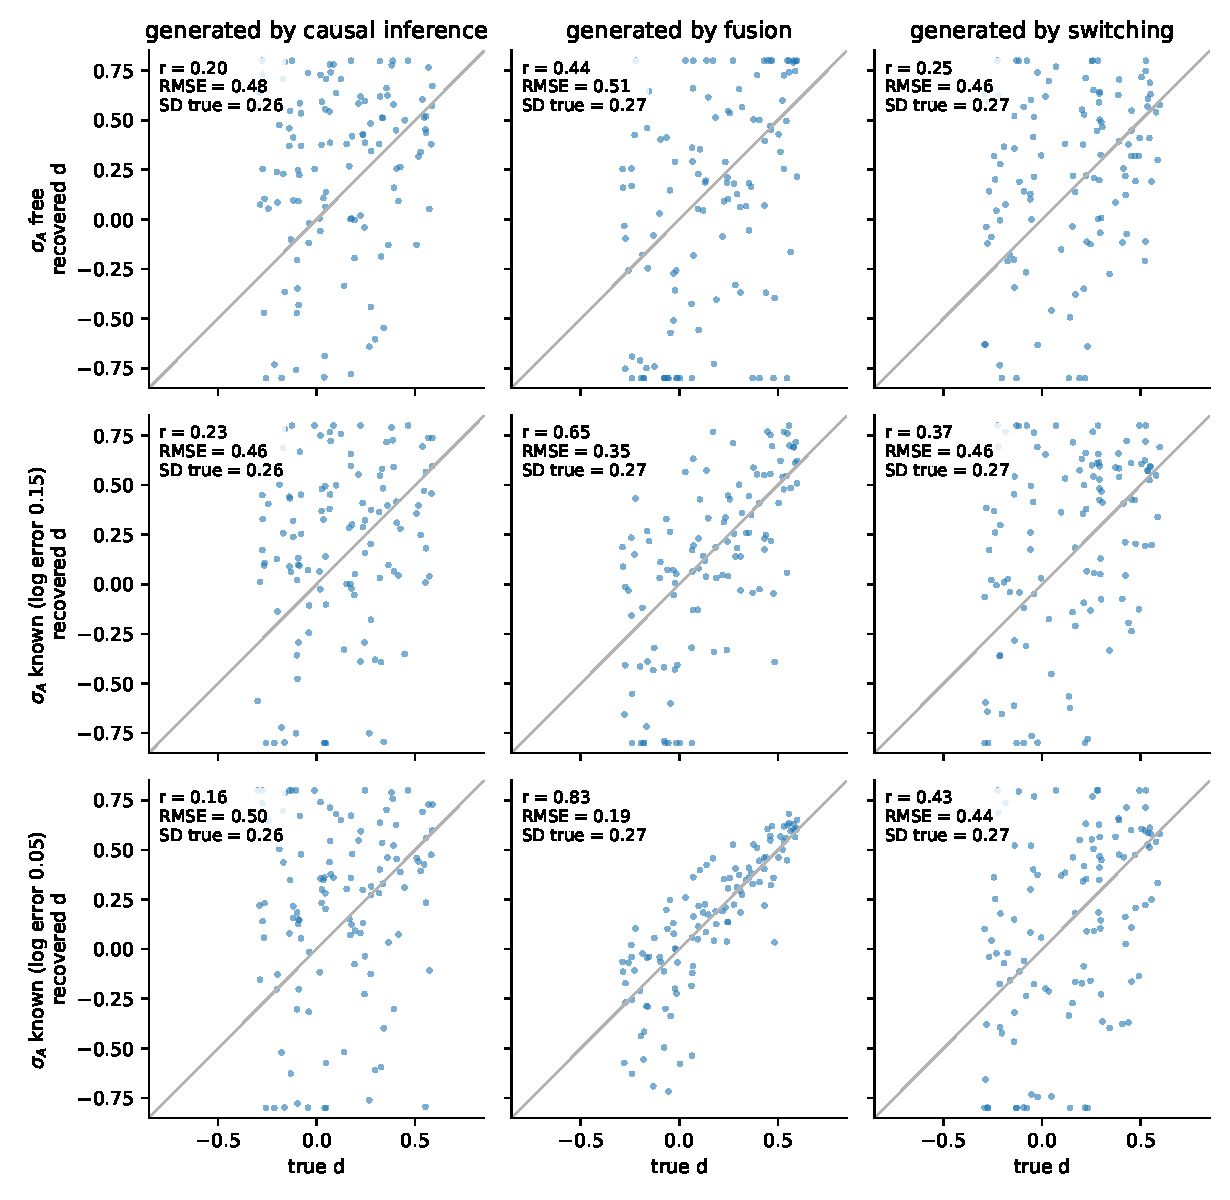
\includegraphics[width=0.6\linewidth]{fig_bias_d.pdf}
\caption{Recovered vs true $d$ (fit with $c$ and $d$ free). Rows: what is known about $\sigma_A$. Only fusion observers with precisely known $\sigma$s give a usable $d$. The $d$-only fit gives the same picture (fusion $r$ = 0.44 / 0.65 / 0.83 across the three scenarios) and underestimates $d$ for CI observers by 0.21--0.26 on average.}
\end{figure}

\noindent The reason is that, once $\sigma_A$ and $\sigma_V$ are known, the fused PSE shift is set by $w_V(1-d)$ times the conflict, so $d$ follows from the size of the shift. In CI and switching, the size of the shift also depends on $\pc$ or $p_\text{switch}$, so a smaller $d$ and a smaller $\pc$ look alike. This is also why AIC picks the $d$ fit for 98\% of fusion observers with $|d| > 0.3$ when $\sigma_A$ is known precisely. A large $d$ is detectable in a fusion observer, but it cannot be measured in the others.

\subsection{Model recovery}
\begin{figure}[H]
\centering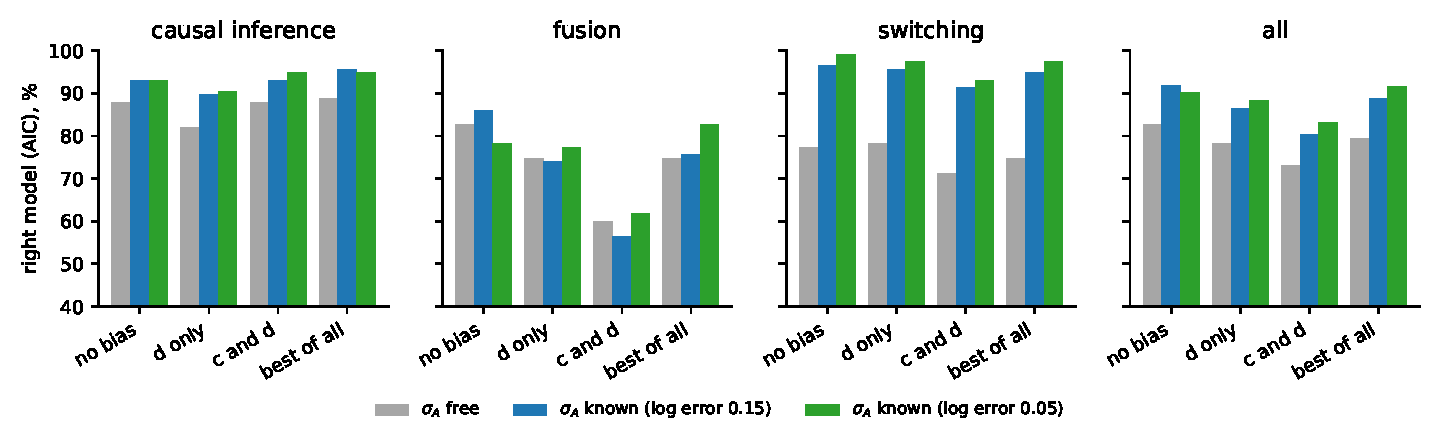
\includegraphics[width=\linewidth]{fig_bias_modelrec.pdf}
\caption{Right model by AIC. ``Best of all'' picks among all nine fits (3 models $\times$ 3 bias variants). Chance is 33\%.}
\end{figure}

\begin{table}[H]
\centering\small
\begin{tabular}{llrrrr}
\toprule
fit & scenario & CI & fusion & switching & all \\
\midrule
no bias & $\sigma_A$ free & 88 & 83 & 77 & 83 \\
        & $\sigma_A$ known, 0.15 & 93 & 86 & 97 & \textbf{92} \\
        & $\sigma_A$ known, 0.05 & 93 & 78 & 99 & 90 \\
\midrule
$d$ only & $\sigma_A$ free & 82 & 75 & 78 & 78 \\
         & $\sigma_A$ known, 0.15 & 90 & 74 & 96 & 86 \\
         & $\sigma_A$ known, 0.05 & 91 & 77 & 97 & 88 \\
\midrule
$c$ and $d$ & $\sigma_A$ free & 88 & 60 & 71 & 73 \\
            & $\sigma_A$ known, 0.15 & 93 & 57 & 91 & 80 \\
            & $\sigma_A$ known, 0.05 & 95 & 62 & 93 & 83 \\
\midrule
best of all & $\sigma_A$ free & 89 & 75 & 75 & 79 \\
            & $\sigma_A$ known, 0.15 & 96 & 76 & 95 & 89 \\
            & $\sigma_A$ known, 0.05 & 95 & 83 & 97 & 92 \\
\bottomrule
\end{tabular}
\caption{Right model by AIC, \% (115--116 participants per model; the SE of a single cell is about 3--4 points).}
\label{tab:modelrec}
\end{table}

\begin{itemize}
\item \textbf{With $\sigma_A$ free,} fusion and switching are mistaken for CI: 17\% and 16\% of the time (no-bias fits).
\item \textbf{With $\sigma_A$ known,} switching is almost always found (97\%). The remaining error is fusion read as CI (10\%).
\item \textbf{Bias terms hurt fusion most.} With $c$ and $d$ free, CI absorbs fusion observers, and fusion recovery drops to 57--62\%.
\item \textbf{Very precise $\sigma$s expose the missing $d$.} With log error 0.05 and no bias terms, recovery falls from 98\% for $0 < d < 0.3$ to 80\% for $d > 0.3$, and fusion overall falls to 78\%. When $\sigma_A$ is known precisely, a large unmodelled $d$ no longer fits. At log error 0.15 the drop is smaller (96\% to 89\%).
\end{itemize}

\subsection{$\pc$}
\begin{table}[H]
\centering\small
\begin{tabular}{lcccccc}
\toprule
 & \multicolumn{2}{c}{no bias} & \multicolumn{2}{c}{$d$ only} & \multicolumn{2}{c}{$c$ and $d$} \\
\cmidrule(lr){2-3}\cmidrule(lr){4-5}\cmidrule(lr){6-7}
scenario & $r$ & RMSE & $r$ & RMSE & $r$ & RMSE \\
\midrule
$\sigma_A$ free & 0.81 & 0.167 & 0.78 & 0.171 & 0.63 & 0.222 \\
$\sigma_A$ known, 0.15 & 0.83 & 0.155 & 0.82 & 0.158 & 0.73 & 0.193 \\
$\sigma_A$ known, 0.05 & 0.88 & 0.127 & 0.83 & 0.156 & 0.78 & 0.176 \\
\bottomrule
\end{tabular}
\caption{$\pc$ recovered by the CI fit for CI participants (true SD 0.25). Mean $\pc$ error of the no-bias fit by true $d$ ($\sigma_A$ known, 0.15): $-0.12$ for $d < 0$, $-0.02$ for $0 \le d \le 0.3$, $+0.02$ for $d > 0.3$. The $d$ fit halves the first ($-0.06$) without lowering the RMSE.}
\end{table}

\section{Noise calibration and presentation order}\label{sec:order}
\texttt{analysis/noise\_calibration\_order\_check.py}. P105's calibration chose noise 1.67, where the unimodal auditory block then measured $\sigma$ 1.6--1.9 instead of the target 0.75. P103 showed the same pattern: calibrated at 1.78, unimodal $\sigma$ 2.3.

\paragraph{What happens.} With the test second, discrimination stays sharp in loud noise. With the test first it falls to chance, with a bias towards calling the second interval longer.
\begin{itemize}
\item \textbf{P105 at 1.67, test second:} ``test longer'' for 4\% of 100\,ms tests and 94\% of 950\,ms tests.
\item \textbf{P105 at 1.67, test first:} 24\% and 38\%.
\end{itemize}
The same pattern appears in every participant except P102 (Table~\ref{tab:order}). It is not a stimulus artefact: PsychoPy's Hamming option only ramps 5\,ms at each end. It matches the known advantage of the standard coming first in duration discrimination (internal-reference account).

\begin{table}[H]
\centering\small
\begin{tabular}{lrrrrrr}
\toprule
 & calibrated & \multicolumn{2}{c}{calibration, \% correct} & \multicolumn{3}{c}{unimodal block at that level, $\sigma$} \\
\cmidrule(lr){3-4}\cmidrule(lr){5-7}
 & level & test first & test second & pooled & test first & test second \\
\midrule
P101 & 0.53 & 58 & 88 & 0.42 & 0.86 & 0.17 \\
P102 & 0.93 & 63 & 77 & -- & -- & -- \\
P103 & 1.78 & 68 & 82 & 2.31 & 3.20 & 0.48 \\
P104 & 1.10 & 59 & 88 & 0.47 & 1.43 & 0.20 \\
P105 & 1.67 & 55 & 92 & 1.58 & 7.8 & 0.03 \\
\bottomrule
\end{tabular}
\caption{Calibration: \% correct at $\pm$0.41 (332/752\,ms) within a factor of 1.4 of the chosen level. Unimodal block: lognormal fits per order (lapse $\le 0.1$). Very large or very small $\sigma$s are poorly determined, because QUEST+ placed those tests at the extremes. P102's unimodal block at the calibrated level was stopped after 8 trials. In a joint fit of all of P102's data, P102 is the one symmetric listener ($\sigma$ 0.60 vs 0.56 at noise 0.5).}
\label{tab:order}
\end{table}

\paragraph{Why the calibration overshot.} The calibration scores \% correct at a fixed $\pm$0.41, pooled over orders. Test-first trials near chance plus test-second trials at about 95\% already give the 70.7\% target. That pooled value barely changes between noise 1 and 2 (P105: about 77\% to 74\%), so the staircases cannot find the level and drift upwards. The unimodal block instead fits one $\sigma$ over both orders and tests of 80--950\,ms. There, the test-first trials stay near chance even at a 9.5-fold difference, which needs a very large $\sigma$.

\paragraph{Starting point, trials and a cap.} Each participant's data were fitted with a $\sigma(\text{noise})$ and a PSE per order, and the calibration was rerun 150 times on that fitted listener:

\begin{table}[H]
\centering\small
\begin{tabular}{lccccc}
\toprule
calibration & P101 & P102 & P103 & P104 & P105 \\
\midrule
before 28 Oct (start 0.3/1.6, 100 per staircase, cap 2.0) & 0.70 & 1.07 & 1.24 & 1.32 & 1.44 (0.94--1.79) \\
both start at 0.5 & 0.61 & 0.93 & 1.06 & 1.20 & 1.36 (0.79--1.71) \\
200 trials per staircase & 0.63 & 1.06 & 1.15 & 1.42 & 1.47 (1.11--1.85) \\
cap 1.5 & 0.64 & 0.91 & 1.03 & 0.98 & 1.17 (0.76--1.41) \\
\textbf{cap 1.2, both start at 0.5 (since 28 Oct)} & 0.64 & 0.84 & 0.95 & 0.89 & 0.99 (0.75--1.11) \\
\bottomrule
\end{tabular}
\caption{Median level reached (80\% range for P105). More trials do not help, the start point helps a little, and the cap does most of the work. The calibration summary now also reports \% correct by order near the chosen level, and warns if test-first is below 60\% and more than 25 points behind test-second.}
\end{table}

\paragraph{Consequence for the models.} With the test second, noise barely changes discrimination: P105's $\sigma$ goes from 0.12 at noise 0.5 to 0.22 at 2.0, P103's from 0.28 to 0.41. The noise manipulation of auditory reliability therefore works mostly through the first interval. The bimodal models (and the simulations above) assume a single $\sigma_A$ per noise level. If the bimodal data show the same order dependence, sharing a pooled unimodal $\sigma_A$ with them may mislead, and the $\sigma_A$ gain in Table~\ref{tab:modelrec} would not carry over.

\section{Limitations}
\begin{itemize}
\item The simulated observers have no order effect, and the $\sigma_A$ penalty assumes the unimodal block measures the $\sigma_A$ that the bimodal task uses (Section~\ref{sec:order}).
\item $\sigma_V$'s error is 0.2 in the $\sigma_A$-free scenario and 0.15 in the $\sigma_A$-known one, so part of the gain may come from $\sigma_V$. In the 28 Oct report, $\sigma_V$ alone (free vs fixed) moved recovery by 11 points, while 0.2 vs 0.15 is a much smaller change.
\item The bias ranges rest on three participants' cross-modal blocks.
\item Fits are BADS local optima, with 3 starts plus the no-bias start. The bound hits for $c$ show a flat likelihood, not a failed optimiser: the same fits recover the model parameters well.
\item Only 70 trials per condition were simulated in the $\sigma_A$-known scenarios. With $\sigma_A$ free, 106 trials gave the same bias recovery as 70.
\end{itemize}

\end{document}
